\documentclass[swedish,a4paper,oneside,12pt, landscape]{scrbook}


%\linespread{0.85}

%\usepackage{bookman}
\usepackage[utf8x]{inputenc}
\usepackage{babel}
\setcounter{tocdepth}{3}

\clubpenalty = 10000 
\widowpenalty = 10000
\usepackage[T1]{fontenc}

\setlength\parskip{\baselineskip}
\setlength\parskip{\medskipamount}
\usepackage{geometry}
\areaset[-3cm]{20cm}{14cm}
%\setlength\parindent{0pt}
%\setlength{\unitlength}{1cm}
%\addtolength{\textheight}{2cm}

\usepackage{bookman}
\usepackage{nopageno}

\usepackage{graphicx}
\usepackage{ae}
%\usepackage{aecompl}
%\usepackage{amssymb}
%\usepackage{amsmath}

\usepackage{tikz}


\begin{document}


\flushleft
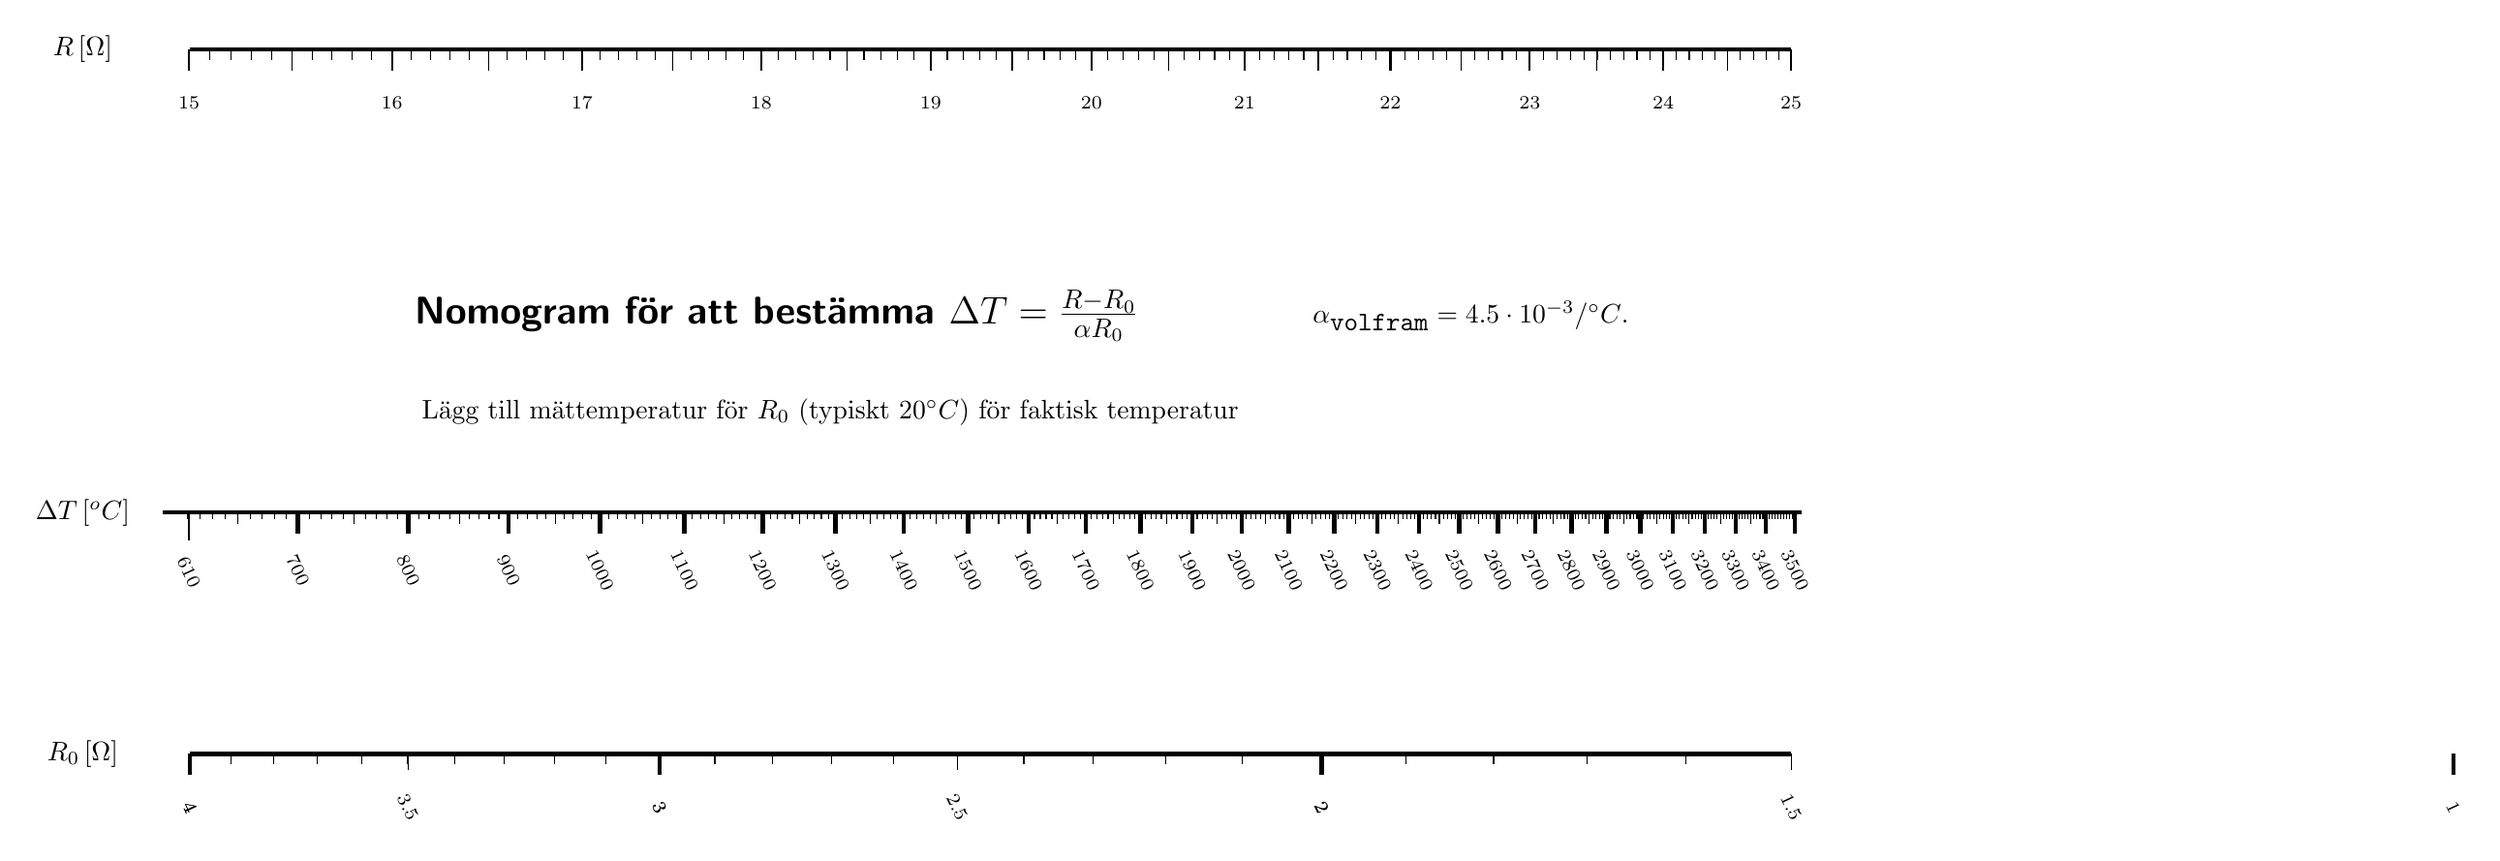
\begin{tikzpicture}[scale=1.4] %[xscale=1.3,yscale=1.3]
%



\draw[ultra thick] (0,0) --(15,0); \node at (-1,0) {$R\, [\Omega]$};
% R
\foreach \x in {15,...,25} {
\node at (67.614/ln 10 *ln \x -79.52, -0.5) {\scriptsize{\x}}; 
\draw[thick] (67.614/ln 10 *ln \x -79.52,-0.2) -- (67.614/ln 10 *ln \x -79.52,0);
}
\foreach \x in {15,15.1,...,25} {
\draw[thin] (67.614/ln 10 *ln \x -79.52,-0.1) -- (67.614/ln 10 *ln \x -79.52,0);
}
\foreach \x in {15,15.5,...,25} {
\draw[thin] (67.614/ln 10 *ln \x -79.52,-0.2) -- (67.614/ln 10 *ln \x -79.52,0);
}
\node at (5.5,-2.5){\Large\textsf{\textbf{Nomogram för att  bestämma $\Delta T=\frac{R-R_0}{\alpha R_0}$ }}};
\node at (12,-2.5){$\alpha_{\texttt{volfram}}= 4.5 \cdot 10^{-3}/ ^\circ C$.};
\node at (6,-3.4){Lägg till mättemperatur för $R_0$ (typiskt $20 ^\circ C$) för faktisk temperatur};

% temp

\draw[ultra thick] (-0.25,-4.34) --(15.1,-4.34); \node at (-1,-4.34) {$\Delta T \, [^o C]$};
\foreach \x in {700,800,...,3500} {
\node[rotate=-65] at ({23.14/ln 10 *ln (\x*0.0045+1) -13.29}, -4.88) {\scriptsize{\x}}; 
\draw[ultra thick] ({23.14/ln 10 *ln (\x*0.0045+1) -13.29},-4.54) -- ({23.14/ln 10 *ln (\x*0.0045+1) -13.29},-4.34);
}


%
\foreach \x in {610,620,...,3500} {
\draw[thin] ({23.14/ln 10 * ln (\x*0.0045+1) -13.29},-4.4) -- ({23.14/ln 10 *ln (\x*0.0045+1) -13.29},-4.34);
}

\foreach \x in {650,750,...,3400} {
\draw[thin] ({23.14/ln 10 * ln (\x*0.0045+1) -13.29},-4.45) -- ({23.14/ln 10 *ln (\x*0.0045+1) -13.29},-4.34);
}
\foreach \x in {1000,1500,...,3500} {
\draw[ultra thick] ({23.14/ln 10 * ln (\x*0.0045+1) -13.29},-4.54) -- ({23.14/ln 10 *ln (\x*0.0045+1) -13.29},-4.34);
}

\foreach \x in {610} {
\node[rotate=-65] at ({23.14/ln 10 *ln(611*0.0045+1) -13.29}, -4.9) {\scriptsize{\x}}; 
\draw[thick] ({23.14/ln 10 *ln(611*0.0045+1) -13.29},-4.6) -- ({23.14/ln 10 *ln(611*0.0045+1) -13.29},-4.34);
}

% R_0
% skala
\draw[ultra thick] (0,-6.6) --(15,-6.6); \node at (-1,-6.6) {$R_0\, [\Omega]$};
%grovmodul med text
\foreach \x in {4,3,...,1} {
\node[rotate=-65] at (-35.21/ln 10 *ln \x +21.2, -7.1) {\scriptsize{\x}}; 
\draw[ultra thick] (-35.21/ln 10 *ln \x +21.2,-6.8) -- (-35.21/ln 10 *ln \x +21.2,-6.6);

}
%Vissa tjocka streck
\foreach \x in {4,3.5,...,1.5} {
\node[rotate=-65] at (-35.21/ln 10 *ln \x +21.2, -7.1) {\scriptsize{\x}}; 

\draw[thin] (-35.21/ln 10 *ln \x +21.2,-6.75) -- (-35.21/ln 10 *ln \x +21.2,-6.6);
}
%Finmodul utan text
\foreach \x in {4,3.9,...,1.4} {

\draw[thin] (-35.21/ln 10 *ln \x +21.2,-6.7) -- (-35.21/ln 10 *ln \x +21.2,-6.6);
}

\end{tikzpicture}
%

\end{document}

